\RequirePackage{fix-cm}

\documentclass[twocolumn,draft,natbib]{svjour3}
\smartqed  % flush right qed marks, e.g. at end of proof

\usepackage{graphicx}


\journalname{Autonmous Robots}
\begin{document}

%%%%%%%%%%%%%%%%%%%%%%%%%%%%%%%%%%%%%%%%%%%%%%%%%%%%%%%%%%%%%%%%%%%%%%%%%%%%%%%%
\title{Atlas RRT Gaussian Process for best-next touch in shape object modelling
  \thanks{This work is supported by EC-FP7-ICT-600918, PacMan.}
}
\subtitle{A probabilistic approach to tactile exploration.}
%\titlerunning{Short form of title}

\author{Carlos J. Rosales         \and
        Claudio Zito              \and
        Federico Spinelli         \and \\
        Jeremy L. Wyatt           \and
        Marco Gabiccini           \and
}

\institute{C. J. Rosales, F. Spinelli, and M. Gabiccini \at
              Centro di Ricerca ``E. Piaggio'', Univ. di Pisa, Italy. \\
              Tel.: +39 (050) 2217050\\
              \email{carlos.rosales@for.unipi.it}           %
           \and
           C. Zito and J. L. Wyatt \at
              Intelligent Robotics Laboratory, Univ. of Birmingham, UK.\\
              Tel.: +44 (0) 121 415 8722\\
              \email{cxz004@cs.bham.ac.uk}              %
}

\date{Received: date / Accepted: date}
% The correct dates will be entered by the editor


\maketitle

%%%%%%%%%%%%%%%%%%%%%%%%%%%%%%%%%%%%%%%%%%%%%%%%%%%%%%%%%%%%%%%%%%%%%%%%%%%%%%%%
\begin{abstract}
Insert your abstract here. Include keywords, PACS and mathematical
subject classification numbers as needed.
\keywords{Active exploration \and 
          Next-best tactile planning \and 
          Object shape modelling}
\end{abstract}

%%%%%%%%%%%%%%%%%%%%%%%%%%%%%%%%%%%%%%%%%%%%%%%%%%%%%%%%%%%%%%%%%%%%%%%%%%%%%%%%
\section{Introduction}
\label{intro}

On object shape modelling:

Implicit e.g. like using a Gaussian Process with theory from \citet{Rasmussen2006Gaussian}. vs Explicit representations. See comparison \citet{Pirri2006About}.

This is also related to what you need to exploit from the shape...

On active exploration with tactile sensing:

Similar work -- \citet{Bjorkman2013Enhancing}

On exploring (probabilistically) implicit manifolds:

AtlasRRT -- \citet{Jaillet2013Path}.

Own previous work -- \citet{Rosales2014Active}.

%%%%%%%%%%%%%%%%%%%%%%%%%%%%%%%%%%%%%%%%%%%%%%%%%%%%%%%%%%%%%%%%%%%%%%%%%%%%%%%%
\section{Equipment abstraction}
\label{sec:equipment}

%%%%%%%%%%%%%%%%%%%%%%%%%%%%%%%%%%%%%%%%%%%%%%%%%%%%%%%%%%%%%%%%%%%%%%%%%%%%%%%%
\section{Object shape representation}
\label{sec:object}


%%%%%%%%%%%%%%%%%%%%%%%%%%%%%%%%%%%%%%%%%%%%%%%%%%%%%%%%%%%%%%%%%%%%%%%%%%%%%%%%
\section{}
\label{sec:equipment}

%%%%%%%%%%%%%%%%%%%%%%%%%%%%%%%%%%%%%%%%%%%%%%%%%%%%%%%%%%%%%%%%%%%%%%%%%%%%%%%%
\begin{acknowledgements}
The authors would like to thank E. Farnioli for the fruitful discussions and 
initial matlab implementations about Gaussian Processes, as well as to G. 
Santaera for the support with the sensorized glove.
\end{acknowledgements}

%%%%%%%%%%%%%%%%%%%%%%%%%%%%%%%%%%%%%%%%%%%%%%%%%%%%%%%%%%%%%%%%%%%%%%%%%%%%%%%%
\bibliographystyle{spbasic}
\bibliography{bib/report}

\end{document}
% end of file

%%%%%%%%%%%%%%%%%%%%%%%%%%%%%%%%%%%%%%%%%%%%%%%%%%%%%%%%%%%%%%%%%%%%%%%%%%%%%%%%
%% HELPS
% \begin{equation}
% a^2+b^2=c^2
% \end{equation}
%
% \begin{figure}
% \centering
%   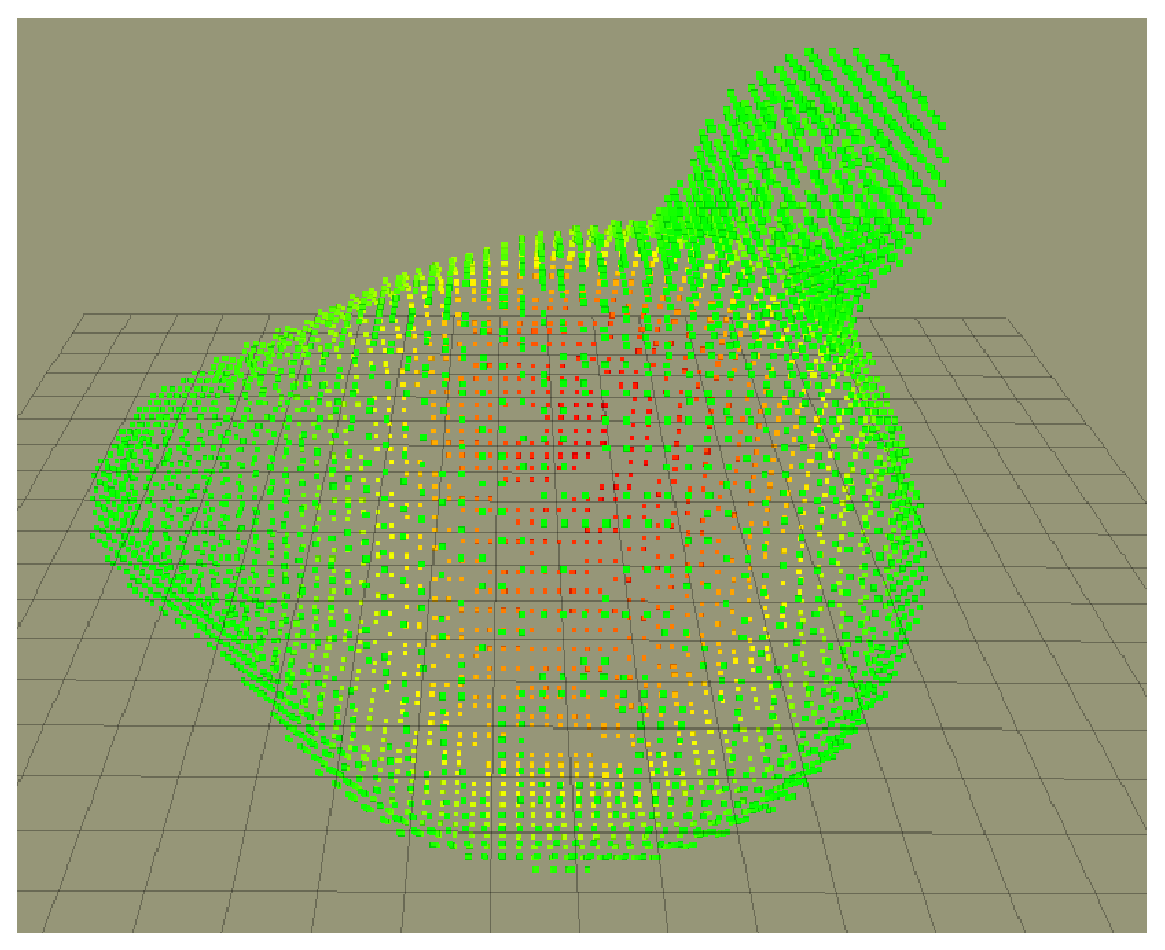
\includegraphics{example.eps}
% \caption{Please write your figure caption here}
% \label{fig:1}
% \end{figure}
%
% \begin{figure*}
% \centering
%   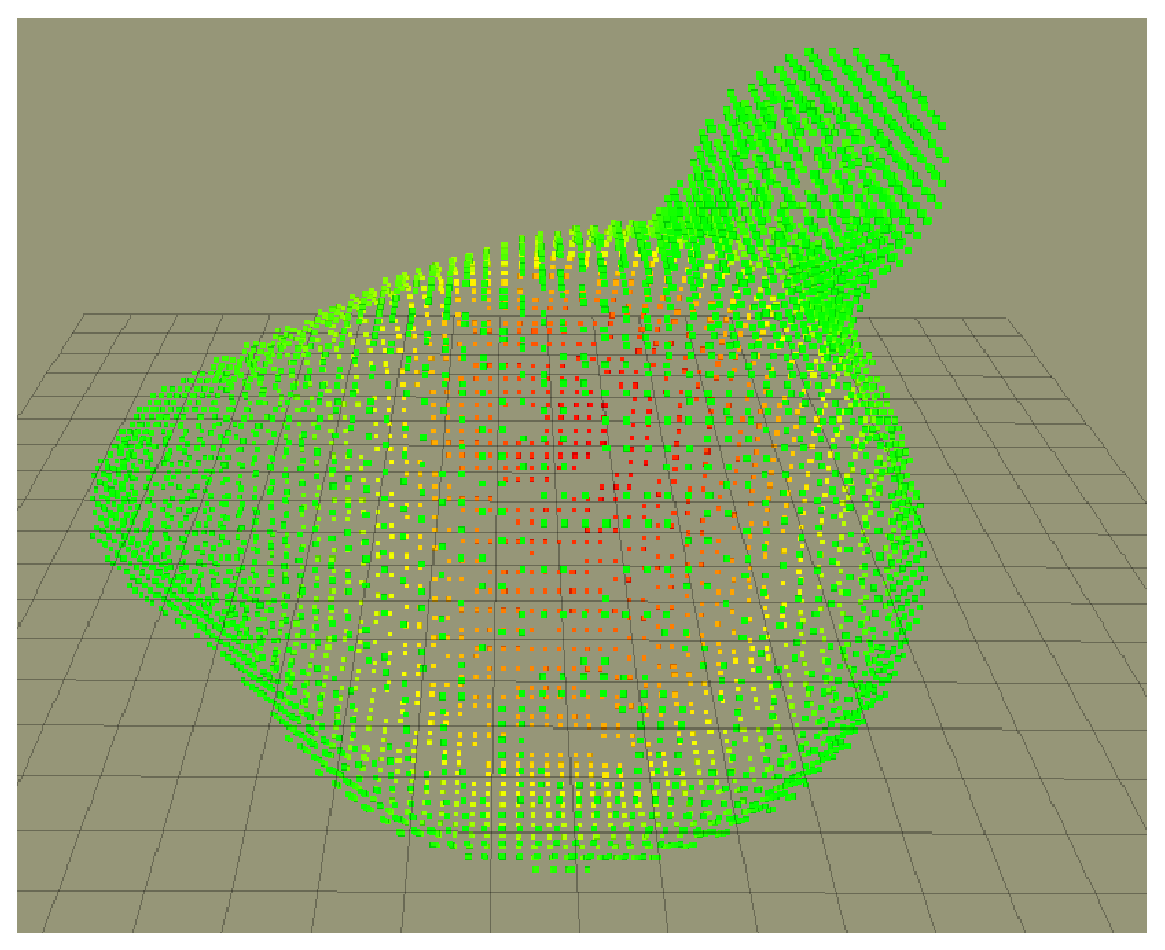
\includegraphics[width=0.75\textwidth]{example.eps}
% \caption{Please write your figure caption here}
% \label{fig:2}
% \end{figure*}
%
% % For tables use
% \begin{table}
% \caption{Please write your table caption here}
% \label{tab:1}
% \begin{tabular}{lll}
% \hline\noalign{\smallskip}
% first & second & third  \\
% \noalign{\smallskip}\hline\noalign{\smallskip}
% number & number & number \\
% number & number & number \\
% \noalign{\smallskip}\hline
% \end{tabular}
% \end{table}
%%%%%%%%%%%%%%%%%%%%%%%%%%%%%%%%%%%%%%%%%%%%%%%%%%%%%%%%%%%%%%%%%%%%%%%%%%%%%%%%